\chapter[SCP-157 幻象猎食者]{
    SCP-157 Mimetic Predator\\
    SCP-157 幻象猎食者
}

\label{chap:SCP-157}

\begin{figure}[H]
    \centering
    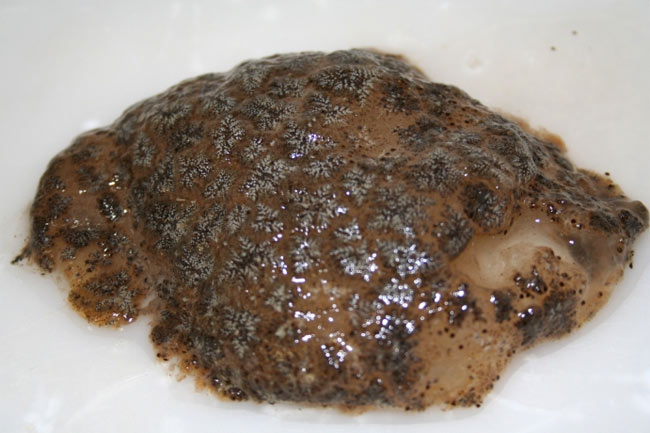
\includegraphics[width=0.5\linewidth]{images/SCP.157.jpg}
    \caption*{一个自然状态下的小型SCP-157群体}
\end{figure}

\bb{项目编号:}SCP-157

\bb{项目等级:}Euclid

\bb{特殊收容措施:}SCP-157在不用于实验时应以其隐生状态存放在干燥的密封容器中。预计SCP-157可在该状态下存活至少10年。实验需要的样品可从容器中取出,并给予水及食物使其恢复为可用状态。

在激活状态下的SCP-157群体处工作的人员不得在SCP-157旁进食、饮水、更衣或在身体表面涂抹任何物质。

批准基金会机动特遣队特工对外界的SCP-157袭击幸存者和目击者进行A级记忆消除。

\bb{描述:}SCP-157是一种此前未知的缓步动物门的微小动物,作为陆生捕食者生活。像其他缓步动物一样,SCP-157对恶劣环境有极强的抵抗力,当没有食物时可进入隐生状态。SCP-157通常表现为由数百万独立个体组成的一团无定形物质。在这种形态下,它可以缓慢地移动和攀爬。

SCP-157群体是捕食性的,会吞噬昆虫和小动物,再用消化酶慢慢溶解猎物。人类及其它大型猎物因为体型太大,难以被吞噬,且SCP-157需要长时间接触目标才能成功进食,所以很少直接被SCP-157群体袭击。该生物发展出了一种替代办法以达成这样的接触。

SCP-157群体有着天生的心灵感应能力。当猎物体积太大,无法直接攻击时,SCP-157群体利用其心灵感应能力表现出猎物想食用、穿戴或涂抹至身体表面的物质的幻象。SCP-157被食用时有剧毒,食用者需要在20分钟内服用{[}编辑]和{[}编辑]的解毒剂,并立刻进行胃部手术以移除被食用的部分。当被涂抹至人类或动物的皮肤时,SCP-157会分泌痲醉剂,使得猎物忽视疼痛并让其留在皮肤上。接下来它将在30分钟至2小时内溶解及消化皮肤。死去的猎物将被SCP-157快速消化,SCP-157进食时将明显成长。SCP-157达到5千克的大小时将分裂成小群体并寻找新的猎物。

同时出现在2个或更多的个体前时,SCP-157的外观不确定——其可能在一人眼中表现为食物,而在另一人眼中表现为衣物。这种情况可作为一种警示以避免与该生物的接触。

\bb{附录:}注意因为其恢复力强的特性,SCP-157可以在被分成小块、煮熟、微波照射等处理后仍保持活力及危险性。

\bb{SCP-157捕获事件:}

\bb{事件157-01} █████ █████,被发现时因为误将SCP-157当做一瓶洗发液抹在头发上导致头皮严重受损。受害者显然对SCP-157的麻醉剂免疫,开始尖叫,吸引了其正在吃点心的妻子的注意。“那是我见过的最奇怪的事情——他把一个五香熏牛肉三明治放在头上,而且那个三明治在吃他!”受害者接受了对化学灼伤的治疗,SCP-157被活捉。受害者及妻子在接受了A级记忆消除后被释放。

\bb{事件157-02} ███████ █████,在其位于██████公司的办公室中被发现,已经部分被SCP-157消化。看起来其认为SCP-157是一双袜子并穿上了它们。受害者在脚掌和小腿基本被溶解后流血致死。

\bb{事件157-03} 对警方报告的例行监听发现了一宗人口失踪案,调查此案的警员观察到一条长沙发缓慢地尝试爬向失踪者的公寓门口。长沙发一开始被警方封锁在区域内;基金会特工随后查明它是一个异常大的SCP-157变种,并收容了该个例。实施了记忆消除。虽然该个例大得足以直接袭击人类,但它还是倾向于使用小型SCP-157群落的手段,用心灵感应能力吸引猎物。
